% Universidade Federal de Itajuba
% Instituto de Matematica e Computacao
%
% Modelo LaTeX para escrita de trabalhos da (Minicurso, Projeto, Relatório)
% para os cursos de Ciencia da Computacao e Sistemas de Informacao, em formato de artigo.
% Insira o nome dos integrantes do trabalho no arquivo configuracao.tex


% Passe, entre os colchetes, a sigla do curso: cco/sin (letras minusculas)
\documentclass[sin]{imc}

% Definicao dos dados do autor do trabalho
% Edite o arquivo 'configuracao.tex'
% Arquivo de configuracao do documento
% Define os dados dos autores do trabalho

% Nome dos integrantes. Deixe as chaves em branco caso não seja usado
\autorNomeA{2023008101 - Eleanderson Ambrozio Jeronimo}
\autorNomeB{2023007089 - Gabriel Barbosa Fernandes}
\autorNomeC{2023005075 - Matheus Lázaro de Lima}
\autorNomeD{2020024371 - Nicole Veronica Pinto dos Santos}
\autorNomeE{ }

% PARA ALTERAR ENTRE SEMINÁRIO E PROJETO FINAL, acesse o arquivo imc.cls, comente a linha 98 e descomente a linha 99

% O titulo do trabalho
\titulo{Middleware para Comunicação Distribuída:Um Estudo do NATS}

% Ano de publicacao do trabalho
\ano{2026}

% Semestre em que foi desenvolvido o trabalho
\mes{1º Semestre}

% Local: nao altere
\local{Itajubá}

% Data da defesa: para fins de preenchimento da folha de aprovacao
% Coloque o mes por extenso, como no exemplo abaixo
%\dataDefesa{23 de novembro de 2021}
 % Nao altere este comando

% Inicio do documento
\begin{document} % Nao altere este comando

% Gera a capa, folha de rosto, ficha catalografica e folha de aprovacao: obrigatorios no texto.
\maketitle % Nao altere este comando

% Secoes do texto: para inserir novas secoes, seguir o mesmo modelo abaixo.
\section{Introdução}
\label{introducao}

A arquitetura proposta baseia-se no middleware NATS, uma tecnologia de mensageria distribuída orientada ao paradigma \textit{publish/subscribe}. O NATS permite comunicação assíncrona de baixa latência, em que produtores publicam eventos e consumidores inscritos recebem mensagens por meio de subjects.

Como evidência prática, este trabalho apresenta um protótipo com comunicação entre processos distribuídos mediada pelo NATS, implementando um modelo cliente-servidor capaz de demonstrar as operações propostas no seminário, incluindo troca de mensagens, alteração remota de arquivos e execução distribuída de cálculos.

















\section{Fundamentação Conceitual}
\label{fundamentacao}


\subsection{Paradigma Publish/Subscribe}

O paradigma \textit{Publish/Subscribe} (Pub/Sub) é um modelo de comunicação assíncrona em que produtores (\textit{publishers}) publicam eventos em canais lógicos, enquanto consumidores (\textit{subscribers}) recebem mensagens associadas aos tópicos de seu interesse. Diferentemente do modelo cliente-servidor tradicional, esse padrão promove desacoplamento entre emissores e receptores.\cite{microsoft_pubsub}

A comunicação é mediada por um intermediário responsável por distribuir eventos aos assinantes adequados, favorecendo escalabilidade e comunicação reativa em sistemas distribuídos, além de reduzir o acoplamento entre componentes e evitar dependências diretas típicas de modelos síncronos, que podem comprometer a flexibilidade e a resiliência do sistema.

No NATS, esse paradigma é implementado por meio de \textit{subjects}, tópicos hierárquicos utilizados para o roteamento eficiente das mensagens.


\subsection{NATS Core}

O NATS Core corresponde à camada básica de mensageria do ecossistema NATS e implementa comunicação leve baseada no paradigma \textit{publish/subscribe}. Seu modelo prioriza simplicidade, baixa latência e alto throughput, oferecendo comunicação nativa muitos-para-muitos (M:N) entre processos distribuídos.

Além do paradigma pub/sub discutido anteriormente, o NATS Core incorpora mecanismos como \textit{request-reply}, para interações do tipo requisição-resposta, e \textit{queue groups}, que permitem distribuir mensagens entre consumidores e balancear carga de processamento.

No que se refere à confiabilidade, o NATS Core opera com semântica \textit{at-most-once}, em que a mensagem é enviada sem persistência nativa ou retransmissão automática, priorizando desempenho e caracterizando o modelo básico de entrega da plataforma.

\subsection{JetStream}
Complementando o modelo básico do NATS Core, o JetStream introduz persistência e streaming, ampliando as garantias de entrega da plataforma.

Por meio de \textit{streams} e \textit{consumers}, permite armazenamento de mensagens, replay de eventos e desacoplamento temporal entre produtores e consumidores, possibilitando que mensagens sejam consumidas mesmo após sua publicação. Além disso, suporta semânticas de entrega \textit{at-least-once} e cenários \textit{exactly-once} baseados em confirmações de processamento.

Segundo a documentação oficial do NATS, o JetStream também suporta replicação baseada em quorum via algoritmo RAFT, fornecendo tolerância a falhas e alta disponibilidade em ambientes distribuídos \cite{nats_jetstream}.

\section{Arquitetura da Tecnologia NATS}
\label{fundamentacao}


\subsection{Componentes}
\label{fundamentacao}
O ecossistema NATS é estruturado a partir de três componentes centrais:

\begin{itemize}

\item \textbf{NATS Server (\textit{nats-server})}: núcleo responsável por gerenciar conexões, realizar o roteamento das mensagens e manter o estado das assinaturas ativas. Sua arquitetura é orientada a baixa latência e processamento eficiente de eventos.

\item \textbf{Clients (Publishers e Subscribers)}: aplicações que interagem com o servidor publicando ou consumindo mensagens. No protótipo desenvolvido, o \textit{publisher} representa o serviço emissor de eventos, enquanto os \textit{subscribers} representam os consumidores dessas respostas.

\item \textbf{Subjects}: tópicos hierárquicos utilizados para endereçamento e roteamento das mensagens (por exemplo, \textit{investimentos.acoes.petr4}). A entrega é baseada no interesse dos assinantes registrados nesses subjects.

\end{itemize}

\subsection{Modelo de Comunicação}
\label{fundamentacao}
O middleware adota um modelo de comunicação assíncrono baseado em troca de mensagens.

\begin{itemize}

\item \textbf{Publish-Subscribe (1:N):} mensagens publicadas em um \textit{subject} são entregues aos assinantes interessados e ativos no momento da publicação, caracterizando o modelo básico de comunicação do NATS.

\begin{figure}[ht]
\centering
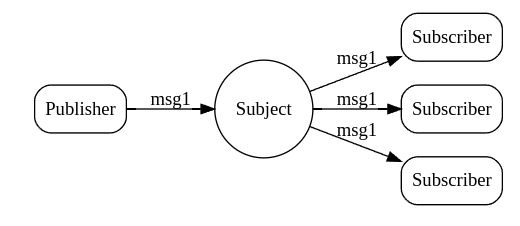
\includegraphics[width=0.75\linewidth]{figs/pubsub.png}
\caption{Modelo Publish-Subscribe no NATS.}
\label{fig:pubsub}
\end{figure}

\item \textbf{Request-Reply (1:1):} padrão construído sobre pub/sub em que um cliente envia uma requisição e recebe resposta por meio de um \textit{reply subject}, viabilizando comunicação orientada a serviços.

\begin{figure}[ht]
\centering
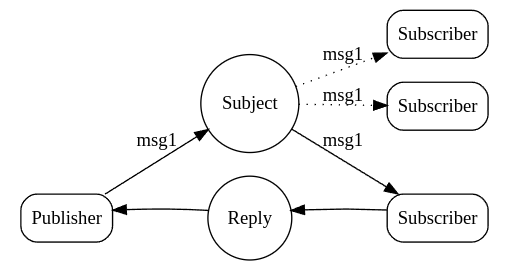
\includegraphics[width=0.75\linewidth]{figs/request-reply.png}
\caption{Modelo Request Reply.}
\label{fig:request-reply}
\end{figure}

\item \textbf{Queue Groups:} múltiplos consumidores compartilham uma mesma assinatura, mas cada mensagem é processada por apenas um deles, permitindo balanceamento de carga e escalabilidade horizontal.

\begin{figure}[ht]
\centering
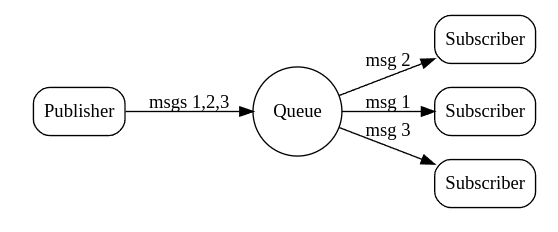
\includegraphics[width=0.75\linewidth]{figs/queue-groups.png}
\caption{Modelo Queue Groups.}
\label{fig:queue-groups}
\end{figure}

\end{itemize}

\subsection{Subjects}

Os \textit{subjects} são os identificadores utilizados pelo NATS para organizar e direcionar a comunicação entre clientes, funcionando como canais lógicos de publicação e subscrição. Esse modelo garante transparência de localidade, já que produtores e consumidores não precisam conhecer a localização uns dos outros.

Eles podem ser estruturados de forma hierárquica por meio do caractere \texttt{.} (\textit{ponto}), permitindo organizar tópicos do mais genérico ao mais específico, como em \texttt{orders.created}. Essa hierarquia é essencial para o roteamento eficiente das mensagens.

O NATS também suporta \textit{wildcards} em subscrições: \texttt{*} (\textit{asterisco}), que representa exatamente um nível da hierarquia, e \texttt{>} (\textit{maior que}), que corresponde a múltiplos níveis subsequentes. Essa flexibilidade permite implementar estratégias como filtragem de mensagens, controle de acesso e otimização do roteamento.

\subsection{Roteamento das mensagens}

O NATS adota um modelo de roteamento baseado em interesse (\textit{interest-based routing}), no qual os servidores mantêm um grafo dinâmico de \textit{subscriptions} \cite{nats_faq}. Esse grafo representa os \textit{subjects} de interesse dos clientes e é propagado entre os nós do cluster. Quando uma mensagem é publicada, ela é encaminhada apenas para os servidores que possuem assinantes interessados no \textit{subject} correspondente, evitando \textit{broadcast} desnecessário e aumentando a eficiência do sistema.


\section{Arquitetura e Implementação do Protótipo}
\label{referencial}

\subsection{Escopo e Arquitetura}

Nesta etapa foi desenvolvido um protótipo utilizando o middleware NATS, com o objetivo de demonstrar a comunicação distribuída entre processos executando em máquinas físicas distintas. O protótipo segue o paradigma de mensageria \textit{publish/subscribe}, permitindo que um cliente envie solicitações e receba respostas processadas por um servidor.


A comunicação entre cliente e servidor ocorre por meio de subjects do NATS, garantindo desacoplamento entre os processos e permitindo escalabilidade para múltiplos clientes ou múltiplos serviços.

\begin{figure}[ht]
\centering
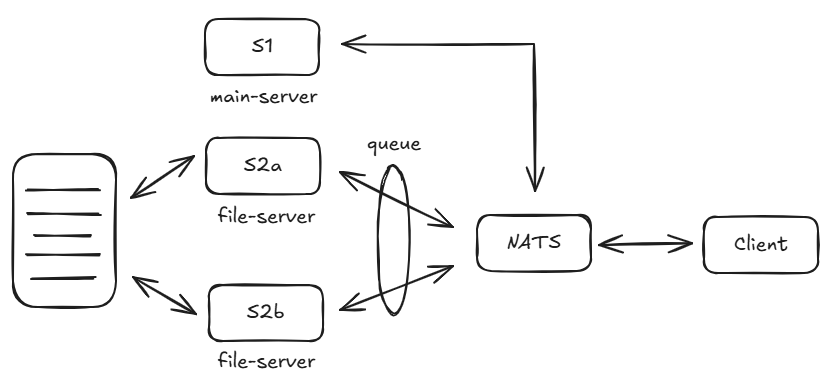
\includegraphics[width=1.0\linewidth]{figs/diagrama_arquitetura.png}
\caption{Diagrama da Arquitetura do Protótipo.}
\label{fig:diagrama_arquitetura}
\end{figure}



\subsection{Operações Implementadas}

\begin{enumerate}
    \item \textbf{Resposta a mensagem de texto}: O cliente publica uma requisição textual em um subject dedicado, que é consumida pelo serviço principal S1. O S1 realiza o parsing da mensagem, processa o conteúdo e retorna uma resposta ao cliente utilizando o padrão request/reply do NATS, validando a troca de mensagens com baixa latência.

    \item \textbf{Alteração de arquivo no servidor}: O cliente envia uma requisição contendo os dados a serem persistidos diretamente ao serviço de arquivos por meio de um subject específico. O processamento é realizado por uma das instâncias S2a ou S2b, configuradas em queue group, garantindo balanceamento de carga entre os servidores. A instância selecionada executa a escrita/atualização do arquivo local e retorna ao cliente o status da operação utilizando o mecanismo de request/reply do NATS.

    \item \textbf{Cálculo de Funções}: O cliente solicita a execução de uma função matemática enviando parâmetros e o tipo de operação desejada. O serviço S1 interpreta a requisição, executa o cálculo e retorna o resultado ao cliente via NATS, utilizando request/reply. Essa operação evidencia o uso do middleware para processamento remoto orientado a mensagens.
    
\end{enumerate}

\subsection{Configuração do Ambiente}

Para a execução do protótipo, foi necessária a configuração do servidor NATS e das dependências da linguagem escolhida.

Inicialmente, o servidor NATS foi executado na máquina responsável pelo broker utilizando o comando: nats-server.

Em seguida, cliente e servidor foram executados em máquinas físicas distintas, conectadas à mesma rede, configurando o endereço IP do servidor NATS para permitir comunicação remota.

Além disso, foi utilizada a biblioteca oficial do NATS para a linguagem escolhida, responsável por estabelecer conexão, publicar mensagens e realizar subscriptions nos subjects definidos.

\section{Evidências Técnicas}

\subsection{Fluxo de Comunicação}

O fluxo de comunicação do protótipo ocorre de forma indireta e desacoplada, sendo mediado pelo middleware NATS, que atua como broker central responsável pelo roteamento das mensagens. O cliente envia requisições publicando mensagens em subjects específicos, e o NATS encaminha essas mensagens aos serviços inscritos nos respectivos canais.

Para operações de texto e cálculo, as mensagens são encaminhadas diretamente ao serviço principal S1 (main-server), que processa a solicitação e retorna uma resposta ao cliente utilizando o mecanismo de request/reply do NATS. Dessa forma, o cliente recebe a resposta sem necessidade de conexão direta com o servidor.

Para operações envolvendo manipulação de arquivos, o cliente publica a requisição diretamente no subject correspondente ao serviço de arquivos. Essa requisição é entregue a apenas uma das instâncias do serviço (S2a ou S2b) devido ao uso de queue group, permitindo balanceamento de carga entre servidores e evitando processamento duplicado. A instância selecionada realiza a operação no armazenamento e retorna o resultado ao cliente por meio do mecanismo de request/reply do NATS. Esse modelo promove maior desacoplamento entre os componentes, além de permitir escalabilidade horizontal e maior tolerância a falhas no serviço de arquivos.

\subsection{Resultados}

Os testes realizados demonstraram que o protótipo implementado com NATS foi capaz de executar corretamente as operações propostas, garantindo comunicação distribuída eficiente entre os componentes. Em todas as requisições enviadas pelo cliente, o sistema retornou respostas estruturadas em formato JSON, contendo código de status, mensagem descritiva e os dados correspondentes ao processamento.


\begin{figure}[ht]
\centering
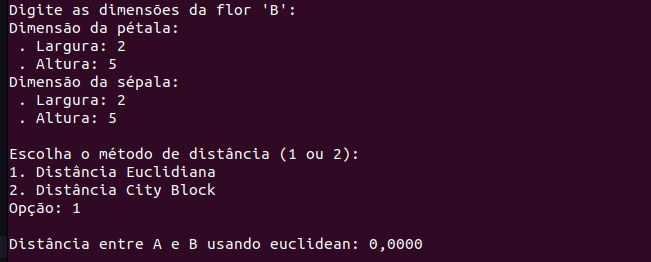
\includegraphics[width=0.75\linewidth]{figs/client-1.png}
\caption{Cálculo de funções.}
\label{fig:resultado}
\end{figure}

\begin{figure}[ht]
\centering
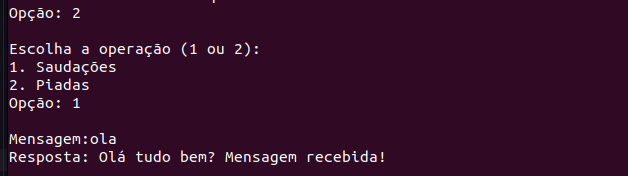
\includegraphics[width=0.75\linewidth]{figs/client-2.png}
\caption{Resposta a mensagem de texto.}
\label{fig:resultado}
\end{figure}

\begin{figure}[ht]
\centering
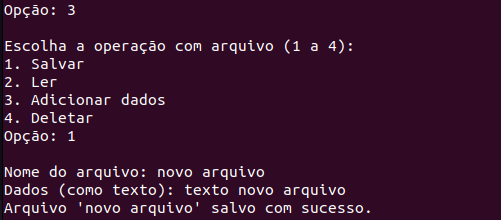
\includegraphics[width=0.75\linewidth]{figs/client-3.png}
\caption{Alteração de arquivo.}
\label{fig:resultado}
\end{figure}


\begin{figure}[ht]
\centering
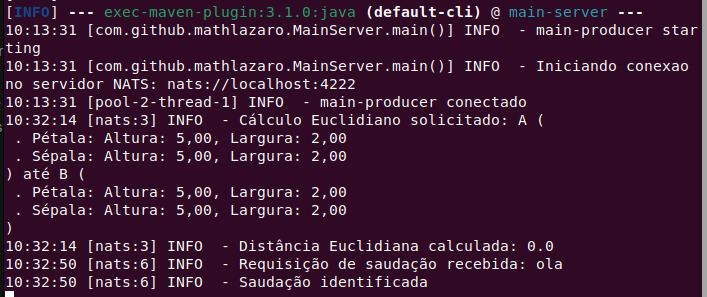
\includegraphics[width=0.75\linewidth]{figs/servidor-mensagem.jpeg}
\caption{Servidor resposta a mensagem.}
\label{fig:resultado}
\end{figure}


\begin{figure}[ht]
\centering
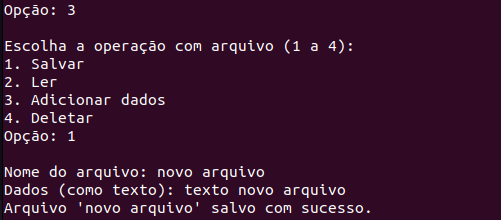
\includegraphics[width=0.75\linewidth]{figs/client-3.png}
\caption{Servidor alteração de arquivo.}
\label{fig:resultado}
\end{figure}


Conforme evidenciado na execução, a operação de envio de mensagem, alteração de arquivo ou cálculo matemático foi concluída com sucesso, retornando mensagens de confirmação como "Operação realizada com sucesso" e status 200, indicando que o fluxo de comunicação baseado em request/reply funcionou corretamente. Dessa forma, os resultados validam que o NATS realizou o roteamento das mensagens de forma adequada e que os serviços distribuídos foram capazes de processar e responder às solicitações conforme o esperado.

\label{ssec:alg}
\section{Uso Prático e Ecossistema}

\subsection{Linguagens e Bibliotecas}
O NATS é agnóstico de linguagem, com suporte oficial e comunitário para dezenas de linguagens, incluindo Go, Python, Java, C/C++, C\#, e JavaScript.

\subsection{Ferramentas Disponíveis}

Para o gerenciamento e monitoramento do cluster, o ecossistema disponibiliza ferramentas oficiais:

\begin{itemize}
\item \textbf{NATS CLI}: administração, testes de publicação/assinatura e gerenciamento do JetStream;

\item \textbf{NATS Server}: servidor distribuído em binário único, adequado para ambientes Docker e Kubernetes.
\end{itemize}

\subsection{Aplicações Reais}
Casos reais de adoção mostram o uso do NATS em aplicações distribuídas com requisitos de desempenho e escalabilidade.
\begin{itemize}

\item \textbf{Finanças e Pagamentos:}
uso em mensageria transacional, processamento de eventos e distribuição de dados em tempo real para sistemas financeiros.

\item \textbf{IoT e Telemetria:}
uso em coleta de métricas, comunicação entre dispositivos distribuídos e arquiteturas edge. Empresas como Siemens aparecem entre casos associados ao ecossistema NATS.

\item \textbf{Microsserviços e Alta Concorrência:}
uso como backbone de comunicação entre serviços distribuídos, com aplicações reportadas em empresas como Capital One, Tinder e outras organizações do ecossistema cloud-native.


\begin{itemize}

\item 
\end{itemize}



\section{Vantagens}
O NATS, por ser escrito em Go, oferece altíssimo desempenho, roteando milhões de mensagens por segundo com latência de microssegundos, próximo ao limite da rede física. É leve e simples, com um único binário sem dependências externas, baixo consumo de RAM e deploy facilitado. Além disso, sua arquitetura em cluster permite auto-descoberta, escalabilidade e auto-reparo, reconfigurando a rede automaticamente em caso de falha de um nó, garantindo alta disponibilidade sem interrupções.

\subsection{Limitações}
O NATS possui limitações como o tamanho restrito das mensagens (1 MB por padrão), sendo mais adequado para mensagens curtas. Também não oferece lógica complexa de roteamento como outros middlewares, utilizando apenas o casamento de strings nos subjects. Além disso, na versão básica (Core), não há persistência nativa — mensagens sem consumidores ativos são descartadas, sendo necessário usar o módulo JetStream para persistência.

\subsection{Comparação com Tecnologias Correlatas}
A Tabela apresenta uma comparação entre o NATS e outras soluções de mensageria amplamente utilizadas, com base em características discutidas por \cite{sharvari2019messaging} e na documentação oficial do NATS \cite{nats_compare}.
\begin{table}[H]
\centering
\caption{Comparação entre middlewares de mensageria}
\begin{tabular}{|l|c|c|c|}
\hline
\textbf{Critério} & \textbf{NATS} & \textbf{RabbitMQ} & \textbf{Kafka} \\ \hline
Latência & Muito baixa & Média/baixa & Média \\ \hline
Persistência nativa & Via JetStream & Sim & Sim \\ \hline
Roteamento complexo & Básico & Avançado & Médio \\ \hline
Escalabilidade & Alta & Média/alta & Alta \\ \hline
Complexidade operacional & Baixa & Média/alta & Alta \\ \hline
\end{tabular}
\label{tab:comparacao_middlewares}
\end{table}

\subsection{Cenários Adequados}
O NATS é indicado para sistemas financeiros e de alta frequência, onde o tempo mínimo de resposta é essencial para distribuir alertas em tempo real. Também é adequado para arquiteturas de microsserviços reativos, atuando como infraestrutura de troca eficiente de mensagens entre serviços, além de aplicações de IoT e telemetria, suportando grandes volumes de pequenos pacotes de dados enviados por sensores e dispositivos conectados.

\subsection{Cenários Não Recomendados}
Não é indicado para transferência de arquivos grandes devido ao limite de tamanho das mensagens, nem para sistemas com transações complexas (ACID), que exigem garantias rigorosas de consistência e rollback. Também não é a melhor escolha para filas de processamento pesado e tarefas de longa duração, onde soluções especializadas em gerenciamento de tarefas podem ser mais adequadas.


\section{Links do Projeto}

\begin{itemize}
    \item Repositório do código-fonte:
    \url{https://github.com/mathLazaro/prototipo-nats}
\end{itemize}





% Estilo da bilbliografia
\bibliographystyle{apalike2_ptBR} % Nao altere este comando

% Bibliografia no formato BibTeX:
% Edite o arquivo 'referencias.bib'
\bibliography{referencias}

% Apendices/Anexos: 
% Se muito necessarios, apendices/anexos devem ser inseridos como \section*{}
% Para inserir estes elementos, seguir o mesmo modelo abaixo.
%\input{nome-do-arquivo}

% Fim do documento
\end{document} % Nao altere este comando
